% -*- root: main.tex -*-

\chapter{Mapowanie obiektowo-relacyjne}
\label{chap:object_relational_mapping}

Mapowanie obiektowo-relacyjne (zwyczajowo określane skrótem ORM od angielskiego terminu \emph{object-relational mapping}) to technologia, która pozwala automatyzować połączenie pomiędzy relacyjnym modelem baz danych, a~paradygmatem programowania zorientowanego obiektowo.~\cite{orm_definition} W~szerokiej perspektywie mapowanie obiektowo-relacyjne może być postrzegane jako próba przełożenia tabelarycznej reprezentacji danych umieszczonej w~pamięci masowej na dowolną reprezentację danych w~pamięci operacyjnej.~\cite{fowler_orm_hate} 

Potrzeba stworzenia mechanizmów ORM to naturalna konsekwencja powstawania aplikacji zorientowanych na przetwarzanie dużej ilości współdzielonych danych. Obsługa dostępu do bazy danych, czyli nieodłączna część współczesnych aplikacji biznesowych, wymaga napisania dużych ilości kodu źródłowego. Kod ten jest powtarzalny pomiędzy poszczególnymi rodzajami danych i~aplikacjami. Jego stworzenie jest pracochłonne, a~nie stanowi żadnej wartości funkcjonalnej dla aplikacji. Mechanizmy ORM w~sposób znaczący redukują ilość kodu niezbędnego do komunikacji z~systemami bazodanowymi. Ich główne zalety to:

\begin{itemize}
	\item Możliwość definiowania modelu danych poprzez tworzenie klas reprezentujących obiekty wykorzystywane w~aplikacji.
	\item Implementacja typowych operacji na danych: tworzenia, aktualizacji, usuwania i~wyszukiwania.
	\item Eliminacja konieczności lub uproszczenie zarządzania połączeniami, sesjami i~transakcjami bazodanowymi.
	\item Zwiększenie bezpieczeństwa aplikacji. Mechanizmy ORM dostarczają narzędzia do ochrony przed atakami typu \emph{SQL Injection}\footnote{SQL Injection (ang. wstrzykiwanie SQL) - typ ataku polegający na wykorzystywaniu specjalnie spreparowanych wartości, które dołączone do szablonu zapytania SQL powodują szkodliwe działanie niezgodne z~intencją programisty.}.~\cite{orm_sql_injection_protection}
	\item Uniwersalne wsparcie dla wielu silników bazodanowych, które mogą różnić się od siebie implementowanymi standardami języka SQL. 
	\item Umożliwienie wymiany środowiska bazodanowego bez konieczności modyfikacji kodu aplikacji.
\end{itemize}

O~powszechnym użyciu mechanizmów ORM w~projektach informatycznych świadczą statystyki:

\begin{itemize}
	\item W~Internecie dostępne są tysiące implementacji mechanizmów ORM o~otwartych źródłach dla dziesiątek różnych języków programowania. Wyszukiwanie frazy \emph{object-relational mapping} w~witrynie \url{http://github.com} zwraca około 45 tysięcy wyników.
	\item Popularnym narzędziem ORM jest biblioteka Hibernate dla języka Java. Wyszukiwanie frazy \emph{\textless artifactId \textgreater hibernate-core \textless /artifactId \textgreater}\footnote{Jest to fraza będąca częścią deklaracji biblioteki Hibernate w~popularnym narzędziu do budowania projektów w~języku Java - Maven.} w~witrynie \url{http://github.com} zwraca około 151 tysięcy wyników.
\end{itemize}

O~popularności mechanizmów ORM świadczy ponadto fakt powstawania oficjalnych standardów mapowania obiektowo-relacyjnego włączanych do specyfikacji języków programowania. Przykładem takiego standardu jest JPA\footnote{Java Persistence API - szerszy opis znajduje się w~sekcji~\ref{sec:jpa}.} dla języka Java.

Mapowanie obiektowo-relacyjne nie jest pozbawione wad. Opanowanie podstaw mechanizmów ORM jest często trudniejsze niż nauka języka SQL. Wynika to ze złożoności takich mechanizmów. Przykładowo na projekt Hibernate ORM przypada ponad milion linii kodu źródłowego. Inną często przytaczaną wadą mapowania obiektowo-relacyjnego jest drastyczny spadek wydajności wynikający z~natury mechanizmów ORM. Prowadzi to do sytuacji, w~których organizacje decydują się na stworzenie własnego, dedykowanego dla danego problemu oprogramowania. Ilość projektów, które wykorzystują systemy mapowania obiektowo-relacyjnego pozwala jednak twierdzić, że wady te są akceptowalne w~obliczu licznych zalet ORM.

\section{Java Persistence API}
\label{sec:jpa}

Java Persistence API to interfejs programistyczny, który ma za zadanie uprościć tworzenie, zarządzanie i~zapisywanie obiektów, które reprezentują dane z~baz relacyjnych.~\cite{jpa_documentation} Interfejs JPA operuje na strukturach POJO\footnote{Plain Old Java Object (ang. dosłownie ,,prosty, stary obiekt Java'') - termin określający zwykły obiekt języka Java, używany jako przeciwieństwo Enterprise Java Bean, czyli specjalnego obiektu, który stosował się do wielu ściśle określonych reguł.}, które dekorowane są adnotacjami umożliwiającymi konfigurację reguł mapowania. Przykład takiego obiektu prezentuje listing~\ref{lst:sample_jpa_pojo}. Adnotacja \verb+@Entity+ określa klasę, która reprezentuje encję danych. Parametr \verb+@Id+ dekoruje identyfikator encji, natomiast \verb+@GeneratedValue+ oznacza, że będzie on ustawiany automatycznie. Adnotacje \verb+@Column+ informują, że dane zmienne będą mapowane na kolumny bazodanowe. Parametr \verb+@ManyToMany+ definiuje relację wiele-do-wielu. 

\begin{verbbox}[\footnotesize]
@Entity
public class User {
    @Id
    @GeneratedValue
    private Integer id;

    @Column
    private String name;

    @Column
    private String surname;

    @Column 
    private String password;

    @ManyToMany
    private List<Item> wishlistItems;

    // getters & setters
}
\end{verbbox}

\begin{figure}[ht!]
	\centering
	\theverbbox
	\caption{Przykładowy obiekt specyfikujący użytkownika w~standardzie JPA.}
	\label{lst:sample_jpa_pojo}
\end{figure}

Definicja encji~\ref{lst:sample_jpa_pojo} nie specyfikuje kompletnego przykładu. Brakuje przede wszystkim wartości konfiguracyjnych, takich jak nazwa tabeli, z~której encja będzie mapowana, nazwy kolumn czy też sposób reprezentacji relacji wiele-do-wielu. W~rzeczywistości JPA nie jest tak czytelene jak sugeruje przedstawiony przykład. Parametry konfiguracyjne zajmują większą część definicji klasy i~zdarza się, że najważniejsza informacja - specyfikacja samego obiektu, który reprezentuje dane - jest mocno przysłonięta.

Na listingu~\ref{lst:sample_jpa_entity_manager} przedstawiono przykładowy kod, który służy do zapisywania użytkownika w~bazie danych. Do obsługi operacji zapisu wykorzystywany jest zarządca encji (\verb+EntityManager+). Za jego pomocą rozpoczynana jest transakcja (\verb+beginTransaction()+), wywoływane jest żądanie utrwalenia obiektu (\verb+persist()+), a~następnie transakcja jest wykonywana (\verb+commit()+).

\begin{verbbox}[\footnotesize]
User user = new User();
// setting field values
EntityManager manager = managerFactory.createEntityManager();
  manager.getTransaction().beginTransaction();
    manager.persist(user);
  manager.getTransaction().commit();
manager.close();
\end{verbbox}

\begin{figure}[ht!]
	\centering
	\theverbbox
	\caption{Przykładowy kod zapisujący użytkownika w~bazie danych w~standardzie JPA.}
	\label{lst:sample_jpa_entity_manager}
\end{figure}

Do najbardziej popularnych implementacji Java Persistence API należą Hibernate ORM, OpenJPA oraz Toplink. Dużą przeszkodą jest fakt, że interfejs JPA nie jest wyczerpująco określony. Opisuje on tylko najbardziej podstawowe operacje na obiektach bazodanowych. Z~jednej strony pozostawia to twórcom bibliotek dużą elastyczność w~kwestii implementacji. Z~drugiej sprawia, że w~przypadku wykonywania operacji bardziej skomplikowanych niż zapisanie i~odczytanie mapowanego obiektu, programista często jest zmuszony sięgać do elementów specyficznych dla danej implementacji JPA. Sprawia to, że większość aplikacji wykorzystujących wymienione biblioteki jest nieprzenośna pomiędzy mechanizmami.

\section{Kundera}
\label{sec:kundera}

Wraz z~pojawieniem się języka CQL pojawiła się szansa wykorzystania istniejących implementacji mechanizmów ORM do przechowywania danych z~użyciem silnika Cassandry. Motywacją do stworzenia takiego rozwiązania jest zwiększenie wydajności istniejących aplikacji bez modyfikacji ich kodu. Minimalna rekonfiguracja aplikacji i~podłączenie jej pod klaster bazodanowy skutkowałyby zwiększeniem wydajności działania aplikacji. Ponadto wykorzystanie istniejących interfejsów mogłoby umożliwić obsługę różnych typów baz danych należących do ruchu NoSQL. 

Przykładem projektu, który wykorzystuje mechanizm ORM do obsługi NoSQLowych baz danych jest Kundera.\cite{kundera_home} Kundera zapewnia implementację mapowania obiektowego zgodną ze standardem JPA 2.0 między innymi dla Cassandry, HBase, MongoDB oraz Neo4j. Dodatkowo biblioteka wspiera obsługę wielu mechanizmów równocześnie.

\subsection{Wydajność}
\label{sec:kundera_performance}

Wyniki pomiarów na stronie domowej projektu Kundera świadczą o~tym, że biblioteka nie wprowadza znacznych narzutów wydajnościowych względem bezpośredniego wykorzystania interfejsu bazy danych. Ważniejsze jest jednak sprawdzenie jak duży narzut wprowadza dostosowanie relacyjnego modelu danych do Apache Cassandry. W~tym celu autor przeprowadził testy porównawcze masowego wstawiania i~pobierania obiektów. Dla każdej z~dwóch operacji zostały przeprowadzone trzy testy. Pierwszy test mierzy czas referencyjny. Jest wykonywany dla zdenormalizowanego modelu Cassandry przedstawionego na diagramie~\ref{tab:denormalized_wishlist}. Drugi test sprawdza czasy dla znormalizowanego modelu zaprezentowanego na diagramie~\ref{fig:er_wishlist}, opisanego w~JPA i~uruchomiony na Cassandrze z~wykorzystaniem biblioteki Kundera. Trzeci test wykorzystuje identyczny opis modelu jak drugi, jednakże wykonywany jest dla silnika MySQL. Wszystkie testy przeprowadzane były jednowątkowo. Czas opóźnień przesyłania danych jest pomijalny, gdyż testy były prowadzone na środowisku lokalnym.

W~trakcie testów mierzony był całkowity czas wykonania danej operacji. Przyjęte zostały następujące założenia:

\begin{itemize}
	\item Liczba użytkowników i~przedmiotów są parametryzowane i~skalowane liniowo.
	\item Liczba przedmiotów, które użytkownik może mieć na swojej liście życzeń zawiera się w~przedziale $[0;10]$.
	\item Odczytywana jest parametryzowalna liczba użytkowników.
\end{itemize}

\noindent Wyniki czasu wstawiania wielu rekordów zostały przedstawione na wykresie~\ref{fig:insert_time_comparison}. Czasy pobierania wielu rekordów zostały zebrane na wykresie~\ref{fig:select_time_comparison}.

\begin{figure}
	\centering
	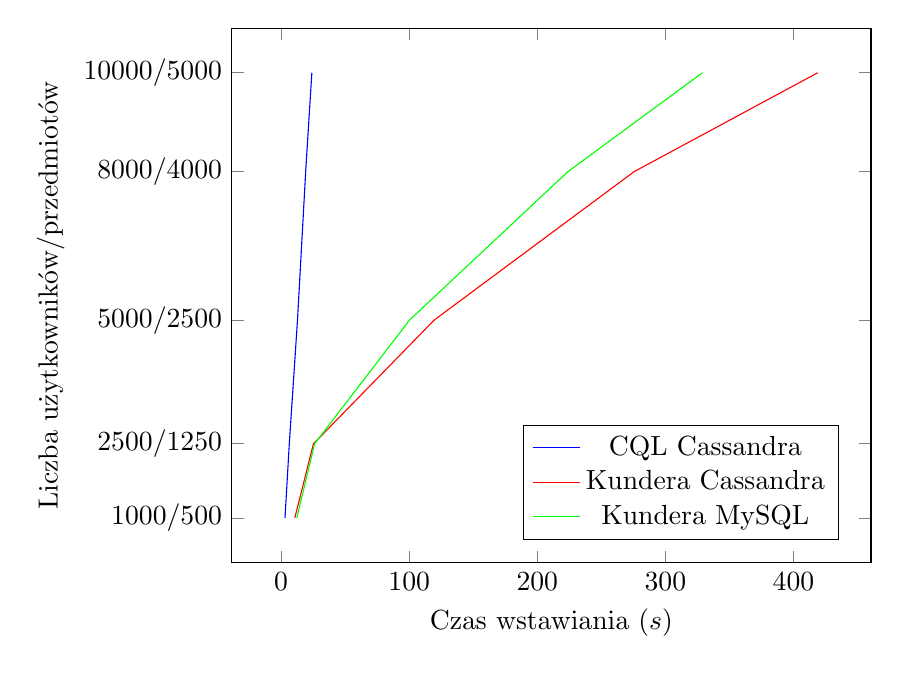
\begin{tikzpicture}
		\begin{axis}[
				width=.8\textwidth,
				xlabel=Czas wstawiania ($s$),
				ylabel=Liczba użytkowników/przedmiotów,
				scaled ticks=false, 
				tick label style={/pgf/number format/fixed},
				ytick={1000, 2500, 5000, 8000, 10000},
				yticklabels={1000/500, 2500/1250, 5000/2500, 8000/4000, 10000/5000},
				legend style={at={(0.95,0.15)},anchor=east}
			]
			\addplot[color=blue] coordinates {
				(23.978, 10000)
				(19.155, 8000)
				(12.762, 5000)
				(6.366, 2500)
				(3.005, 1000)
			};
			\addlegendentry{CQL Cassandra}

			\addplot[color=red] coordinates {
				(418.915, 10000)
				(275.532, 8000)
				(119.453, 5000)
				(25.213, 2500)
				(10.657, 1000)
			};
			\addlegendentry{Kundera Cassandra}

			\addplot[color=green] coordinates {
				(328.915, 10000)
				(223.823, 8000)
				(100.23, 5000)
				(26.119, 2500)
				(12.232, 1000)
			};
			\addlegendentry{Kundera MySQL}
		\end{axis}
	\end{tikzpicture}

	\caption{Porównanie czasu wstawiania wielu rekordów.}
	\label{fig:insert_time_comparison}
\end{figure}

\begin{figure}
	\centering
	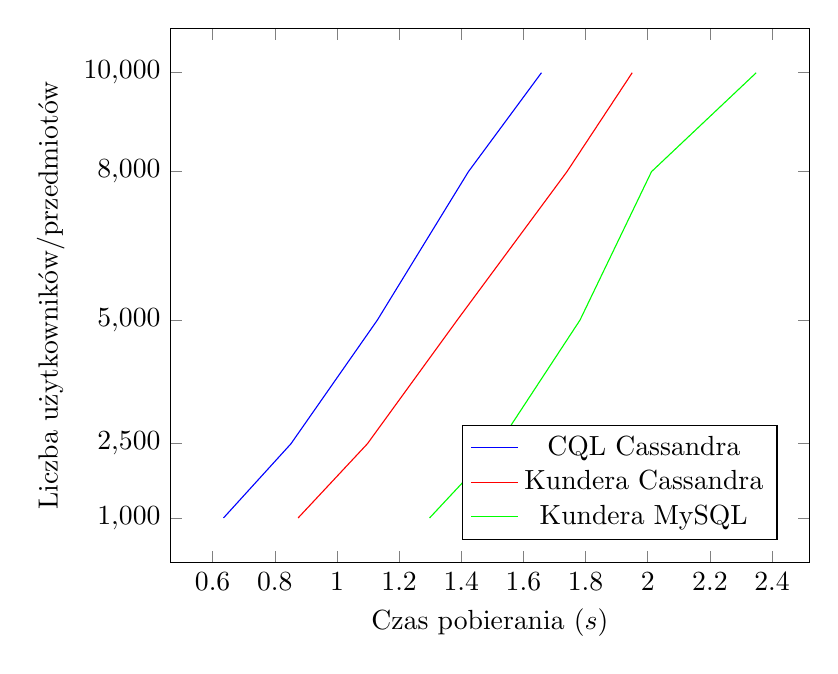
\begin{tikzpicture}
		\begin{axis}[
				width=.8\textwidth,
				xlabel=Czas pobierania ($s$),
				ylabel=Liczba użytkowników/przedmiotów,
				scaled ticks=false, 
				tick label style={/pgf/number format/fixed},
				ytick={1000, 2500, 5000, 8000, 10000},
				legend style={at={(0.95,0.15)},anchor=east}
			]
			\addplot[color=blue] coordinates {
				(1.658, 10000)
				(1.423, 8000)
				(1.130, 5000)
				(0.852, 2500)
				(0.635, 1000)
			};
			\addlegendentry{CQL Cassandra}

			\addplot[color=red] coordinates {
				(1.95, 10000)
				(1.74, 8000)
				(1.387, 5000)
				(1.098, 2500)
				(0.875, 1000)
			};
			\addlegendentry{Kundera Cassandra}

			\addplot[color=green] coordinates {
				(2.349, 10000)
				(2.012, 8000)
				(1.782, 5000)
				(1.521, 2500)
				(1.298, 1000)
			};
			\addlegendentry{Kundera MySQL}
		\end{axis}
	\end{tikzpicture}

	\caption{Porównanie czasu pobierania wielu rekordów.}
	\label{fig:select_time_comparison}
\end{figure}

Wyniki zebrane na wykresie~\ref{fig:insert_time_comparison} pokazują, że wykorzystanie mechanizmów mapowania obiektowo-relacyjnego dla bazy danych Cassandra jest bardzo złym wyborem. Narzut związany z~konwersją modelu danych do postaci relacyjnej jest tak duży, że w~praktyce pojedynczy węzeł Cassandry osiąga gorsze wyniki zapisu niż baza danych MySQL. Zmiana silnika bazodanowego dla istniejącego kodu nie tylko nie poprawi wyników wydajnościowych, ale może wręcz spowodować spowolnienie działania aplikacji. Jedynym zyskiem z~takiego rozwiązania będzie możliwość wykorzystania natywnego mechanizmu klastrowania węzłów Cassandry. Dzięki temu wyeliminowany zostanie pojedynczy punkt awarii systemu. Ten sam efekt można jednak uzyskać stosując rozwiązania dedykowane dla relacyjnych baz danych. Przykładami takich systemów mogą być MySQL Cluster CGE dla bazy danych MySQL oraz Oracle RAC dla baz Oracle Database Enterprise Edition.

Potencjalnym zastosowaniem mapowania obiektowo-relacyjnego dla bazy danych Cassandra są środowiska integracyjne dla wielu aplikacji. Wykorzystując homogeniczny model danych można odwoływać się do różnych silników bazodanowych. W~bibliotece Kundera istnieje takie rozwiązane. Zostało nazwane Polyglot Persistence\footnote{Polyglot Persistence (dosłowne tłumaczenie to ,,zapis poliglotyczny'') - opis mechanizmu znajduje się na stronie \url{https://github.com/impetus-opensource/Kundera/wiki/Polyglot-Persistence}.}. W~praktyce dostosowanie modelu danych ORM do istniejących schematów baz danych jest problematyczne.  

Wykres~\ref{fig:insert_time_comparison} demonstruje jak ogromną przewagę szybkości przy zapisie posiada poprawnie zaprojektowany model danych Apache Cassandra. Przypuszczalnie osiągnięty czas mógłby być jeszcze lepszy, gdyż ograniczenie wydajności zapisu nastąpowało prawdopodobnie po stronie klienta testowego. Zgodnie ze specyfikacją Apache Cassandra jest w~stanie obsługiwać bez opóźnień znacznie więcej jednoczesnych żądań zapisu.

Czasy pobierania listy życzeń użytkownika przedstawione na wykresie~\ref{fig:select_time_comparison} nie różnią się znacząco od siebie. Przewaga szybkości pobierania danych z~wykorzystaniem CQL ponownie wynika z~zastosowania lepszego modelu danych. Denormalizacja pól encji \emph{Item} pozwala pominąć pobieranie dla każdego użytkownika dodatkowego wiersza z~bazy danych. 

\section{Wnioski z~badania wydajności}
\label{sec:cassandra_orm_performance_summary}

Na podstawie wyników przeprowadzonych badań można wnioskować, że mechanizmy mapowania obiektowo-relacyjnego nie nadają się do wykorzystania przez bazę danych Apache Cassandra. Wynika to z~faktu, że mechanizmy te wspomagają normalizację i~zachowywanie relacji między encjami, natomiast efektywne modelowanie dziedziny danych w~Cassandrze dąży do denormalizacji i~maksymalnego uproszczenia zależności pomiędzy obiektami.

Drastyczna różnica szybkości zapisu danych w~modelach zoptymalizowanym i~niezoptymalizowanym świadczy o~tym, że do efektywnego modelowania dziedziny w~Apache Cassandra niezbędne są: wiedza na temat sposobu przechowywania danych przez tę bazę oraz podejmowanie świadomych wyborów. Dostarczone przez ORMy mechanizmy mogą wyłącznie spowolnić korzystanie z~Cassandry.

Podczas badania wydajności autor natrafił również na problemy z~przenośnością kodu źródłowego pomiędzy różnymi systemami bazodanowymi. Wykonanie operacji wstawiania partii danych w~bazie relacyjnej oraz Cassandrze wymagało modyfikacji kodu źródłowego aplikacji testowej. W~relacyjnej bazie danych nie można było ukończyć testu wstawiania i~pobierania danych wykorzystując jedynie elementy zdefiniowane w~JPA. Pomimo wielokrotnej zmiany konfiguracji w~pewnym momencie testu dochodziło do całkowitego zablokowania puli połączeń. Dopiero przejście do transakcji bezstanowej zdefiniowanej w~Hibernate ORM\footnote{Hibernate ORM - środowisko aplikacyjne implementujące standard JPA dla baz relacyjnych. Zdefiniowana w~ramach tego środowiska transakcja bezstanowa nie jest częścią interfejsu JPA, a~więc nie może być wspierana przez Kunderę.} umożliwiło zakończenie testu.

Opisane problemy z~przenośnością kodu mogą być następstwem fundamentalnych różnic pomiędzy relacyjnymi systemami bazodanowymi a~Apache Cassandrą. Przykładowo transakcja, czyli jedno z~podstawowych pojęć związanych z~zapytaniami w~języku SQL, nie istnieje w~systemie Cassandra. Dostosowanie implementacji do interfejsu mapowania obiektowo-relacyjnego wymaga sztucznego blokowania zapytań po stronie klienta, co prowadzi do wystąpienia niepotrzebnych opóźnień i~nadmiernego wykorzystania mechanizmów synchronizacji wielowątkowej. Z~drugiej strony brak lub nieodpowiednie wykorzystanie transakcji w~przypadku bazy relacyjnej prowadzi do błędów zapytań. 

Wyniki badań nie świadczą o~niemożliwości implementacji mapowania obiektowego dla Cassandry. Dla optymalnej wydajności należy jednak zastosować rozwiązane dedykowane:

\begin{itemize}
	\item Definiowanie modelu powinno być skoncentrowane wokół wewnętrznej reprezentacji danych w~Cassandrze. W~stosunku do mapowania obiektowo-relacyjnego kluczowe są aspekty obniżenia istotności relacji i~wsparcie dla operacji denormalizacji z~poziomu interfejsu.
	\item Mapowanie powinno w~prosty i~transparentny sposób udostępniać realizację poprawnych wzorców modelowania. Przykładowo lista wartości powinna móc być zamodelowana przynajmniej na dwa sposoby: jako kolumna typu list lub jako lista kolumn o~nazwach zawierających wartości listy. Mapowanie obiektowe dla Cassandry powinno umożliwiać wymienienie fizycznej struktury danych bez zmiany wykorzystującego ją kodu źródłowego.
	\item Mapowanie obiektowe dla Cassandry powinno być proste. Język CQL, w~porównaniu do SQL, ma prostą składnię i~nie udostępnia wielu operacji. Ponadto skomplikowany mechanizm mapowania mógłby niekorzystnie kontrastować z~wydajną bazą danych. Przykładem nieczytelnego mapowania z~dużą liczbą opcji konfiguracyjnych może być pole encji opisane w~JPA przedstawione na listingu~\ref{vrb:awful_orm}.
\end{itemize}

\begin{verbbox}[\footnotesize]
	@ManyToMany
	@JoinTable(name = "wishlist", 
	           joinColumns = {
	               @JoinColumn(name = "userId", 
	                           referencedColumnName = "userId") },
	           inverseJoinColumns = {
	             { @JoinColumn(name = "itemId", 
	                           referencedColumnName = "itemId") },
	           foreignKey = @ForeignKey(name = "userId_fk"), 
	           inverseForeignKey = @ForeignKey(name = "itemId_fk"))
	private Set<Item> wishlistItems = new HashSet<Item>();
\end{verbbox}

\begin{figure}[ht!]
	\centering
	\theverbbox
	\caption{Przykład nieczytelnego mapowania obiektowo-relacyjnego.}
	\label{vrb:awful_orm}
\end{figure}

\section{Hibernate OGM}
\label{sec:hibernate_ogm}

Alternatywnym rozwiązaniem, które dostarcza implementacji Java Persistence API dla baz NoSQL jest Hibernate Object/Grid Mapper (OGM). Hibernate OGM wykorzystuje silnik projektu ORM o~tej samej nazwie. Niestety, aktualne wydanie (wersja \textbf{4.1.0.Beta5}) wspiera wyłącznie silniki Infispan, Ehcache, MongoDB oraz Neo4j. 

Rozwiązanie to jest jednak interesujące z~punktu widzenia dalszego rozwoju pracy. Według mapy przyszłych wydań Hibernate OGM w~wersji 4.2 wprowadzi wsparcie dla silnika bazy danych Apache Cassandra.~\cite{hibernate_ogm_roadmap} 

\section{Koncepcja mapowania dla Cassandry}
\label{sec:om_for_cassandra_concept}

W~większości rozwiązań ORM encja modelu danych jest opisywana jako definicja klasy, której obiekty reprezentować będą instancję tej encji. Rozważmy listing~\ref{vrb:jpa_denormalization_theory}, który przedstawia hipotetyczne dostosowanie standardu JPA do denormalizacji dla modelu~\ref{tab:denormalized_wishlist}.

\begin{verbbox}[\footnotesize]
	@Table(name = "wishlist")
	class Wishlist {
	    @Id(type = IdType.PARTITION_KEY) 
	    private String userId;
	    @Denormalize(clustering_keys = { "itemId" }, 
	                 fields = { "name", "price" })
	    private Item item;
	}
\end{verbbox}

\begin{figure}[ht!]
	\centering
	\theverbbox
	\caption{Hipotetyczny przykład dostosowania definicji JPA do denormalizacji.}
	\label{vrb:jpa_denormalization_theory}
\end{figure}

W~powyższym przykładzie denormalizacja jest modelowana jako zdegenerowany przypadek relacji jeden-do-jednego. Przypisanie zmiennej \emph{item} do obiektu klasy \emph{Wishlist} i~utrwalenie tego obiektu w~bazie danych spowoduje uzupełnienie wartości kolumn \emph{itemId}, \emph{name} oraz \emph{price} w~tabeli \emph{wishlist}. Po pobraniu obiektu klasy \emph{Wishlist} z~bazy danych przechowywany reprezentant klasy \emph{Item} posiada tylko część informacji. Takie rozwiązanie posiada istotną wadę. Podczas korzystania z~mechanizmu nie można jednoznacznie stwierdzić czy brak uzupełnienia pola \emph{desc} w~obiekcie klasy \emph{Item} jest spowodowany tym, że opisu faktycznie brakuje, czy też operacje dokonywane są na niekompletnym (zdenormalizowanym) obiekcie. Rozwiązaniem pozbawionym tej wady jest denormalizacja jawna przedstawiona na listingu~\ref{vrb:jpa_explicit_denormalization_theory}.

\begin{verbbox}[\footnotesize]
	@Table(name = "wishlist")
	class Wishlist {
	    @Id(type = IdType.PARTITION_KEY) 
	    private String userId;

	    @Id(type = IdType.CLUSTERING_KEY)
	    private String itemId;

	    @Column(name = "name")
	    private String name;

	    @Column(name = "price")
	    private String price;
	}
\end{verbbox}

\begin{figure}[ht!]
	\centering
	\theverbbox
	\caption{Hipotetyczny przykład zastosowania denormalizacji jawnej w~JPA.}
	\label{vrb:jpa_explicit_denormalization_theory}
\end{figure}

Denormalizacja jawna posiada jednak inne wady. Przede wszystkim model nie podaje, że kolumny \emph{itemId}, \emph{name} oraz \emph{price} powinny pochodzić od instancji klasy \emph{Item}. Ponadto użytkownik mechanizmu musi pamiętać o~ręcznym wypełnieniu pól, co jest z~kolei narażone na błędy. Eleganckie połączenie tych dwóch opcji nie jest możliwe w~języku Java. 

Ze względu na mechanizm metaklas w~Pythonie stworzono eleganckie i~proste implementacje ORM dla relacyjnych baz danych. Dwa najpopularniejsze mechanizmy to Django ORM\footnote{Django ORM - część platformy Django, która odpowiada za operacje bazodanowe. Dokumentacja jest dostępna pod adresem \url{https://docs.djangoproject.com/en/dev/topics/db/}.} oraz SQLAlchemy\footnote{Strona domowa projektu jest dostępna pod adresem \url{http://www.sqlalchemy.org}.}. Wykorzystując metaklasy osiągalne jest stworzenie mapowania o~interfejsie wymienionych mechanizmów, który rozwiązuje problem zasygnalizowany w~przypadku języka Java. Ilustruje to listing~\ref{vrb:sql_alchemy_like_denormalization}.

\begin{verbbox}[\footnotesize]
	class Wishlist(Model):
	    userId = TextField(partition_key=True)
	    item = DenormalizedField(relates=Item, 
	                             clustering_keys=['itemId'], 
	                             fields=['name', 'price'])

	w = Wishlist()
	w.item = Item(id='1', name='n', price='10.0')
	id = w.item_itemId    # id equals '1'
	name = w.item_name    # name equals 'n'
	price = w.item_price  # price equals '10.0'
	i = w.item            # exception raised
\end{verbbox}

\begin{figure}[ht!]
	\centering
	\theverbbox
	\caption{Hipotetyczny przykład denormalizacji w~mapowaniu w~języku Python.}
	\label{vrb:sql_alchemy_like_denormalization}
\end{figure}

Dzięki metaklasom można dokonać następujących modyfikacji modelu \emph{Wishlist}:

\begin{itemize}
	\item Dla każdej instancji \emph{DenormalizedField} automatycznie dodać do klasy pola, które będą przechowywać zdenormalizowane wartości. W~przykładzie definicja klasy została rozszerzona o~pola \emph{item\_itemId}, \emph{item\_name}, \emph{item\_price}.
	\item Każdą instancję \emph{DenormalizedField} zamienić na właściwość tylko do zapisu, która automatycznie ustawia wartości zdenormalizowanych pól.
\end{itemize}

Dzięki takim modyfikacjom możliwe jest ustawianie wartości zdenormalizowanych pól poprzez podawanie całej instancji obiektu \emph{Item}, jak w~listingu~\ref{vrb:jpa_denormalization_theory}. Jednocześnie pobieranie wartości z~obiektu możliwe jest tylko poprzez odwołania do zdenormalizowanych pól. Nie da się pomylić ze sobą zdenormalizowanych i~pełnych instancji klasy \emph{Item}.